\def\theTopic{Readings 1}


\begin{center}
{\bf {\large Descriptive Statistics}}
\end{center}


Data is everywhere.  We take for granted the fact that our smart
phones, smart TV's and other hi-tech gadgets store
huge amounts of data about us.  We have quickly become used to being
able to call up all sorts of information from the web. 
To handle data we first have to distinguish several types of data
which are handled and plotted differently.

As an example, suppose that we want to filter out spam messages before
they hit your email inbox.  We can keep track of several attributes
of an email, and each email will have its data on a single line in the
data file (one line is  called a ``{\bf case}'' or a  ``record''). It
may look like this:

\begin{table}[ht]
\centering
\begin{tabular}{rrrrl}
  \hline
 spam & num\_char & line\_breaks & format & number \\ 
  \hline
   0 & 21.70 & 551 &html& small \\ 
   0 & 7.01 & 183 &html& big \\ 
   1 & 0.63 &  28 &text& none \\ 
   0 & 2.45 &  61 &text& small \\ 
   0 & 41.62 & 1088 &html& small \\ 
 \vdots&\vdots&\vdots&\vdots&\vdots\\
   0 & 15.83 & 242 &html& small \\ 
   \hline
\end{tabular}
\end{table}

Where the {\bf variable} in each column tells us:\vspace{-.8cm}
\begin{list}{}{}
  \item [spam] is 1 if the message is known to be spam, 0 otherwise.
  \item [num\_char] counts the length of the message in thousands.
  \item [line\_breaks] counts the number of lines of text.
  \item [format] is either ``html'' or ``text''.
  \item [number] is small if text contains a number $< 1 $ million,
    big if a number over 1 million is included, and none otherwise. 
\end{list}

We will divide variables into two main types:
\begin{list}{}{}
\item [\bf Categorical variables] tell us about some attribute of the
  case which is not numeric, for example: hair color or favorite
  sport.  The categories can be numeric (like zip codes) if it makes
  no sense to ``average'' them together.


\item [\bf Quantitative variables] are numbers which can be averaged
  together. They can be integers( like counts) or precise measurements like
  milliliters of beer in a stein.\vspace{1.5in} 
\end{list}


\begin{center}
{\bf {\large  Data summaries vary with data type}}
\end{center}

\begin{list}{}{}
\item [\bf Categorical variables] are summarized with tables like
  this:

\begin{tabular}{rr}
  \hline
html &  13 \\ 
text &  37 \\ 
   \hline
\end{tabular}

 which says that 13 of the messages were in html format, and 37 were
 plain text.  We could also say that 26\% ($= 13 / 50 \times 100\%$)
 of the emails were in html format. 

\item [\bf Quantitative] variables are summarized with measures of
  center (mean or median) and spread, and sometimes with quartiles.
  \begin{list}{}{}
  \item [mean] or ``average'' is found by summing all values and
    dividing by the size of the sample ( we label sample size as $n$).
    With a ``sample'' of values, we call the first one $x_1$, the
    second $x_2$, and so forth, and we call the mean ``x bar'' which
    is defined as
   $$\xb = \frac{x_1 + x_2 + \cdots x_n}{n}$$
  For the number of characters in the emails, we get 
   $$\xb = \frac{21.7 + 7.0 + \cdots + 15.8}{50} = 11.598.$$
  \item [median] is a number which has half the values below it and
    half above it.  It is not affected by extreme values in the way
    that the mean is.  The number of characters in an email has some
    large values which inflate the mean, but the median is smaller at
    6.89 thousand characters.
  \item [first quartile] labeled $Q_1$, has one fourth of the values
    below it and three-fourths above. It is also called the 25$^{th}$
    percentile. 
  \item [third quartile] labeled $Q_3$, has three fourths of the values
    below it and one-fourth above.  It is also called the 75$^{th}$
    percentile. 
  \item [Inter-Quartile Range] or IQR, is the distance between the
    first and third quartiles.  It is a measure of {\bf spread} of the
    values.  For the 'numbers of characters' data, $Q_1$ is 2.536 and $Q_3$ is
    15.411, so $IQR = 15.411 - 2.536 = 12.875$.
  \item [Standard Deviation] labeled $s$ is roughly the average
    distance from each point to the mean of the sample.  We do not
    expect you to compute it, but the formula is
      $$ s = \sqrt{\frac{(x_1-\xb)^2 + (x_2-\xb)^2 + \cdots+ (x_n-\xb)^2}{n-1}}$$
    which, for the data we are considering, is 13.125.\\
    It is an important measure of {\bf spread}.
  \end{list}
\end{list}
\newpage

\begin{center}
{\bf {\large  Plotting Data}}
\end{center}

 As with numeric summaries, the type of data determines the
 appropriate plot. \vspace{-.5cm}
\begin{list}{}{}
\item [\bf Categorical variables] are plotted using a bar
  chart. (Note, one could use a pie chart, but then it is much harder
  to compare two areas of the pie than with the bar chart.)
  For a more interesting example, we'll consider the admissions rate
  of applicants  to UC-Berkeley grad school in 1973 separated by
  gender. (Gender is categorical and so is ``admitted or  rejected'',
  so the plot allows us to compare one categorical variable split by
  another. This seems more interesting than just looking at one
  variable -- like admission rates for all applicants.)

  \begin{center}
  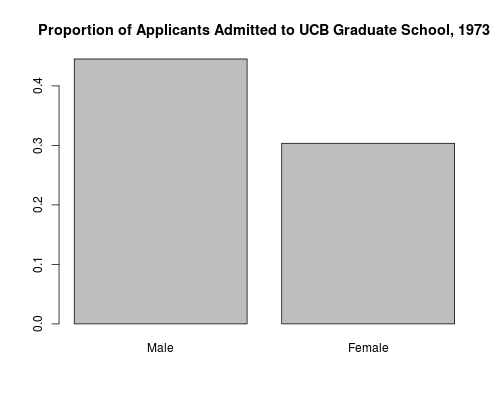
\includegraphics[width = .45\linewidth]{../plots/UCBadmissions.png}
  \end{center}
  
\item [\bf Quantitative variables] are plotted with dot plots, histograms,
  density plots, and boxplots.

  \begin{list}{}{}
  \item [\bf dot plots] represent each point with a dot above the number
    line. This works well with small sample sizes.  If the data are
    too close together to distinguish, we might stack them up to
    remove any overlap. \vspace{-1cm}
%% plot(x=email50$num_char, y = rep(1,50), xlab = "1000 Characters",
%% ylab = "", bty= "n",yaxt="n", cex = 2, pch = 16, col =
%% rgb(0,0,1,alpha = .3))
%% dev.copy(png,"plots/dotplotDemo1.png",height = 200, width = 500);dev.off()

  \begin{center}
  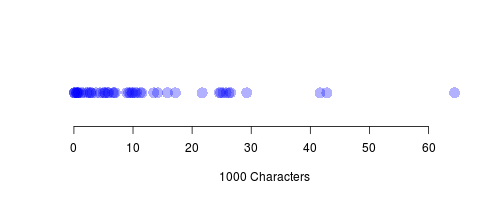
\includegraphics[width = .8\linewidth]{../plots/dotplotDemo1.png}
  \end{center}

  \item [\bf histograms] divide the axis into ``bins'' and count the
    numbers of points falling into each bin.  The height of each bin might
    show the count (frequency) of values in the bin or the proportion
    (relative frequency) for the bin.  These plots work with moderate
    to large sized data sets.  Choosing the best number of bins can be
    hard. \vspace{-.4cm}
%% hist(email50$num_char, xlab = "1000 Characters", main = "")
%% dev.copy(png,"histogramDemo1.png",height = 300, width = 500);dev.off()
  \begin{center}
  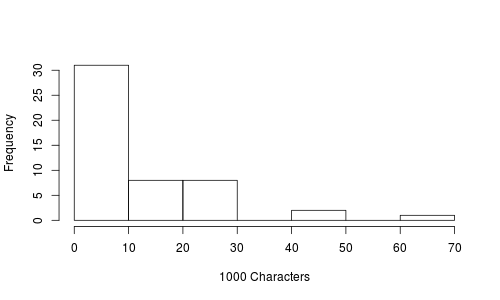
\includegraphics[width = .6\linewidth]{../plots/histogramDemo1.png}
  \end{center}


  \item [\bf density plots] are basically like smoothed off
        relative frequency histograms. \vspace{-.4cm}

%% plot(density(email50$num_char), xlab = "1000 Characters", main = "")
%% dev.copy(png,"densityDemo1.png",height = 300, width = 500);dev.off()
  \begin{center}
  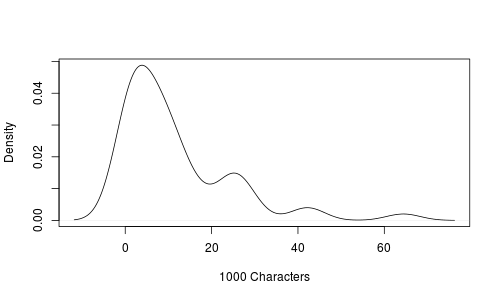
\includegraphics[width = .6\linewidth]{../plots/densityDemo1.png}
  \end{center}

   \item [\bf box-and-whisker plots] show the quartiles of the
     distribution, making a box from $Q_1$ to $Q_3$ (median is also $Q_2$), and
     then showing whiskers which extend to the minimum and maximum
     value. If those extremes are too far out, the whisker usually
     stops at the last point within 1.5 $\times$ IQR's of either
     $Q_1$ or $Q_3$ and flags points beyond 1.5 $\times$ IQR as
     ``outliers'', or unusual points.  
     Half of the data will be included in the box, and half will be
     outside the box. \vspace{-1cm}
%% boxplot(email50$num_char, horizontal = TRUE, xlab = "1000 Characters", main = "")
%% dev.copy(png,"boxplotDemo1.png",height = 200, width = 500);dev.off()
  \begin{center}
  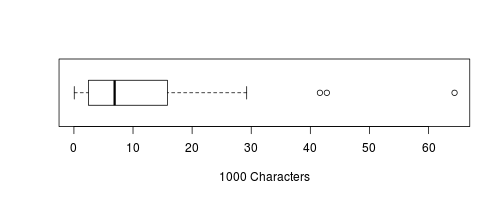
\includegraphics[width = .8\linewidth]{../plots/boxplotDemo1.png} \vspace{-.5cm}
  \end{center}

\end{list}
\end{list}

%%  barplot(prop.table(apply(UCBAdmissions,1:2,sum),2)[1,])
%% title("Proportion of Applicants Admitted to UCB Graduate School, 1973")
%% dev.copy(png,"classes/stat216/TR-F2015/coursePa/plots/UCBadmissions.png",height = 400, width = 500);dev.off()


One more idea is important in describing a sample of quantitative
values is the {\bf skew} of a distribution of values.  \\
  A distribution is skewed if the histogram tapers off to one
  side. For example, the num\_char variable above shows strong right
  skew because the histogram and density plots taper down to the
  right, and the boxplot has a long ``right tail'' (longer whisker to
  right and outliers to right).
\\
 If those same plots look roughly the same on each side, we say the
 data  are ``symmetrically distributed'' rather than saying ``unskewed''.

